\documentclass[12pt,a4paper]{article}
\pdfminorversion=7

% ----- PACKAGES -----
\usepackage[utf8]{inputenc}
\usepackage{graphicx}
\usepackage{geometry}
\usepackage{setspace}
\usepackage{hyperref}
\usepackage{fancyhdr}
\usepackage{titlesec}
\usepackage{booktabs}
\usepackage{multirow}
\usepackage{pgfplots}
\usepgfplotslibrary{groupplots}
\pgfplotsset{compat=1.18}
\usepackage[maxbibnames=3,minbibnames=1,maxcitenames=2,mincitenames=1,style=numeric-comp,backend=biber]{biblatex}
\addbibresource{references.bib}

\geometry{margin=1in}
\setstretch{1.2}
\setlength{\headheight}{14.5pt}
\pagestyle{fancy}
\fancyhf{}
\rhead{Project Report}
\lhead{\leftmark}
\rfoot{Page \thepage}

\title{
    \textbf{Advanced Information Retrieval}\\[0.2cm]
    \large Fine-Tuning and Transferability in Legal Information Retrieval\\[0.2cm]
    \normalsize Group Number: 27\\[0.3cm]
    \normalsize Repository: \href{https://github.com/rhabichl/Advanced-Information-Retrieval}{rhabichl/Advanced-Information-Retrieval}\\[0.15cm]
    \normalsize Adapter: \href{https://huggingface.co/krapfi/Qwen3-Embedding-8B-Ger-Legal}{krapfi/Qwen3-Embedding-8B-Ger-Legal}\\[0.3cm]
}
\author{
    Raphael Habichler\thanks{student-id: 12419578, Role: Data Processing \& Fine-tuning} \and
    Mark Sesko\thanks{student-id: 12114879, Role: Evaluation \& Analysis} \and
    Paul Brandstätter\thanks{student-id: 12212566, Role: Dataset Preparation \& Documentation}
}
\date{\today}

\titleformat{\section}{\large\bfseries}{\thesection}{1em}{}
\titleformat{\subsection}{\normalsize\bfseries}{\thesubsection}{1em}{}

\begin{document}
\pagestyle{empty}
\pagenumbering{roman}
\maketitle
\newpage
\pagenumbering{arabic}
\pagestyle{fancy}

\section{Abstract}
This project tests whether an embedding model fine-tuned on one legal system transfers to others.
We fine-tune Qwen3-Embedding-8B \cite{qwen3embedding} on German legal query-document pairs and evaluate the baseline and fine-tuned model on German, Austrian, and Chinese legal retrieval datasets.
We report Recall@k, Precision@k, and nDCG@k.
The fine-tuned model improves retrieval on German data, but we do not observe clear transfer to Austrian or Chinese data.

\section{Introduction}
Legal information retrieval is important for searching laws and cases.
However, labeled training data is often available only for some jurisdictions.
Our research question is: Can a legal embedding model fine-tuned on German law effectively retrieve relevant documents in other jurisdictions (Austrian and Chinese law)?
If transfer works, we can build better retrieval systems in low-resource settings without collecting large new training datasets.

In this project we focus on an embedding-based retrieval setup.
Both queries and documents are mapped into the same vector space, and we rank documents by similarity to a query.
This approach is attractive because it supports fast retrieval once document embeddings are precomputed.
The main question is whether fine-tuning on one legal system helps retrieval in another legal system, especially across different languages.

\section{Related Work}
GerDaLIR provides a large benchmark for German legal retrieval \cite{wrzalik-krechel-2021-gerdalir}.
LeCaRDv2 provides a benchmark for Chinese legal case retrieval \cite{li2023lecardv2}.
We build on Qwen3-Embedding-8B \cite{qwen3embedding} and evaluate transfer across datasets and languages.

Our setup is a bi-encoder style retrieval model.
Compared to cross-encoders, bi-encoders typically trade some accuracy for efficiency, because documents can be embedded once and reused.
Fine-tuning is commonly used to improve the embedding space for a specific domain.
However, it is unclear if fine-tuning on one legal domain and language generalizes to different legal systems and languages.

\section{Experiments}
\subsection{Datasets}
We use three datasets.
German data comes from GerDaLIRSmall (test split) \cite{wrzalik-krechel-2021-gerdalir}.
Chinese data comes from LeCaRDv2 (test split) \cite{li2023lecardv2}.
Austrian data is a synthetic dataset built from Austrian legal documents where we generate queries from documents.

The three datasets differ in important ways.
German and Chinese datasets contain query-document relevance labels that can include multiple relevant documents per query.
The Austrian dataset in our setup is closer to a one-to-one matching problem, because each generated query is linked to one source document.
This makes the Austrian results harder to compare directly to German and Chinese, but it still gives a signal about transfer.

Our Austrian dataset creation follows a similar idea to the dataset construction outlined in the GerDaLIR work \cite{wrzalik-krechel-2021-gerdalir}, in the sense that we build a structured corpus and then create query-document pairs for retrieval experiments.
In practice, the Austrian Open Data interface is difficult to use and the scraped texts contain many formatting and quality issues.
We expect that this poor data quality is a major reason for the weak performance on the Austrian dataset.

\subsection{Model and Fine-Tuning}
We use Qwen3-Embedding-8B \cite{qwen3embedding} as the baseline embedding model.
We use the SentenceTransformers framework for both embedding creation and fine-tuning.
We fine-tune the model on German query-document pairs using a LoRA adapter (PEFT) with 8-bit quantization.
Training was done on an NVIDIA H200.
We use a contrastive ranking objective (multiple negatives) to increase similarity of matching query-document pairs and decrease similarity to other documents.

We use LoRA because it is memory efficient and allows updating only a small number of trainable parameters.
This is important for large embedding models.
We keep the base model fixed and train low-rank updates on attention projection layers.
The final output is a lightweight adapter that can be shared and loaded on top of the base model.

\subsection{Workflow}
We first download all datasets from Hugging Face.
We then generate embeddings for all queries and documents with our embedding generation script (\texttt{generate\_embeddings.py}).
After that, we train a LoRA adapter on cleaned German query-document pairs with \texttt{finetune\_lora.py}.
Finally, we evaluate retrieval by randomly sampling 1000 queries and ranking them against the full corpus.

For embedding generation, we truncate texts to a fixed maximum length (1024 characters in our scripts) to control memory and runtime.
We normalize embeddings so that the dot product behaves like cosine similarity.
We store embeddings as pickled data frames with document IDs, which keeps evaluation reproducible and avoids recomputing embeddings for every run.

\subsection{Retrieval and Evaluation}
For each query, we embed the query and all candidate documents and rank documents by dot product similarity.
We report Recall@k, Precision@k, and nDCG@k for \(k \in \{1,5,10,20,50,100\}\).
For German and Chinese datasets, we evaluate on a random sample of 1000 queries.
For Austrian data, each query has one matching document, and retrieval is evaluated against the full Austrian candidate set.

Our evaluation uses a simple brute-force retrieval over the full corpus embeddings.
This is computationally heavy but easy to implement and avoids indexing effects.
In practical systems one would use an approximate nearest neighbor index, but the ranking quality at top-k should be comparable if the index is accurate.

\section{Results}
\subsection{German (GerDaLIRSmall)}
Fine-tuning on German improves all metrics across all \(k\), with the largest gains at larger \(k\).
This supports that the LoRA adapter learns German legal retrieval patterns.

We observe the typical pattern that Recall@k increases with larger \(k\), while Precision@k decreases because more non-relevant documents are included.
The increase in nDCG@k indicates that relevant documents are not only found more often, but also ranked higher after fine-tuning.

For example, Recall@100 increases from 0.5066 to 0.7361, and nDCG@100 increases from 0.2863 to 0.3748.
The full German metrics are shown in Appendix Table~\ref{tab:results-german}.

\subsection{Austrian (synthetic)}
On Austrian data, performance is very low for both models.
We see only small changes after German fine-tuning, and the improvements are not consistent across \(k\).
This suggests that German fine-tuning does not reliably transfer to this synthetic Austrian setup.

One possible reason is that the Austrian queries were generated and may not match real search behavior.
Another reason is that Austrian legal language and structure can differ from German training data, even if the language is similar.
Because the task is closer to matching a query back to its source document, small wording differences can have a large impact.
We also observed that the Austrian Open Data interface and scraped texts are noisy and sometimes poorly formatted, which likely hurts both embedding quality and evaluation reliability.

Overall, the values remain close to zero, and the fine-tuned model does not consistently improve the ranking.
The full Austrian metrics are shown in Appendix Table~\ref{tab:results-austrian}.

\subsection{Chinese (LeCaRDv2)}
On Chinese data, the fine-tuned model is slightly worse than the baseline on most \(k\).
We do not see positive transfer from German to Chinese in this setup.
This aligns with the idea that cross-lingual and cross-jurisdiction transfer is difficult without multilingual adaptation or Chinese training data.

The Chinese metrics show relatively high Precision@k and nDCG@k in absolute terms.
This is due to the dataset definition and relevance structure, and it also suggests that the base model already provides strong multilingual embeddings.
Fine-tuning only on German can shift the embedding space toward German legal patterns and may slightly harm Chinese ranking.

For example, nDCG@100 decreases from 0.8579 to 0.8407.
The full Chinese metrics are shown in Appendix Table~\ref{tab:results-chinese}.

\newpage
\section{Conclusion}
We fine-tuned Qwen3-Embedding-8B on German legal pairs and evaluated transfer to Austrian and Chinese retrieval.
We find clear improvements on German test data.
We do not find clear improvements on Austrian or Chinese datasets, and Chinese performance slightly decreases after German fine-tuning.
Overall, our results suggest that domain and language transfer is limited in this setting, and that additional multilingual training data or adaptation methods would likely be needed.

In other words, fine-tuning helps when the evaluation setting matches the training setting.
Once the domain changes (different legal system) or the language changes (Chinese), the gains disappear.
This is a useful result because it shows that a strong base embedding model already generalizes reasonably well, but domain-specific tuning can make the model more specialized.

For future work, we would extend training with multilingual legal pairs and evaluate transfer again.
We would also test training on a mix of German and Austrian data to see if small amounts of in-domain Austrian pairs can improve results.
Finally, we would add an approximate nearest neighbor index for faster retrieval and evaluate whether it matches brute-force rankings at top-k.

\section*{Limitations and Risks}
Our Austrian dataset is synthetic and may not match real user queries.
Cross-language transfer may require explicit multilingual training.
Legal retrieval systems can reflect bias in training data and should not be used as a substitute for legal advice.

Our evaluation uses random sampling of queries, so results can vary slightly across runs.
We also rely on truncation to a fixed text length, which may remove important legal details in long documents.
Finally, we only evaluate a single fine-tuning setup and set of hyperparameters, so there may be better configurations that we did not explore.

Overall, the results should be interpreted as a controlled experiment that tests one clear transfer setting.
Even though we do not see transfer to Austrian and Chinese here, this does not mean transfer is impossible.
It suggests that transfer is not automatic, and that additional data or adaptation steps are needed when moving to a different jurisdiction or language.

\clearpage
\appendix
\section{Visualization of Results}
Figure~\ref{fig:curves} visualizes Recall@k and nDCG@k for baseline and fine-tuned models on all three datasets.
This makes it easier to compare trends across \(k\) than tables alone.

\begin{figure}[h]
\centering

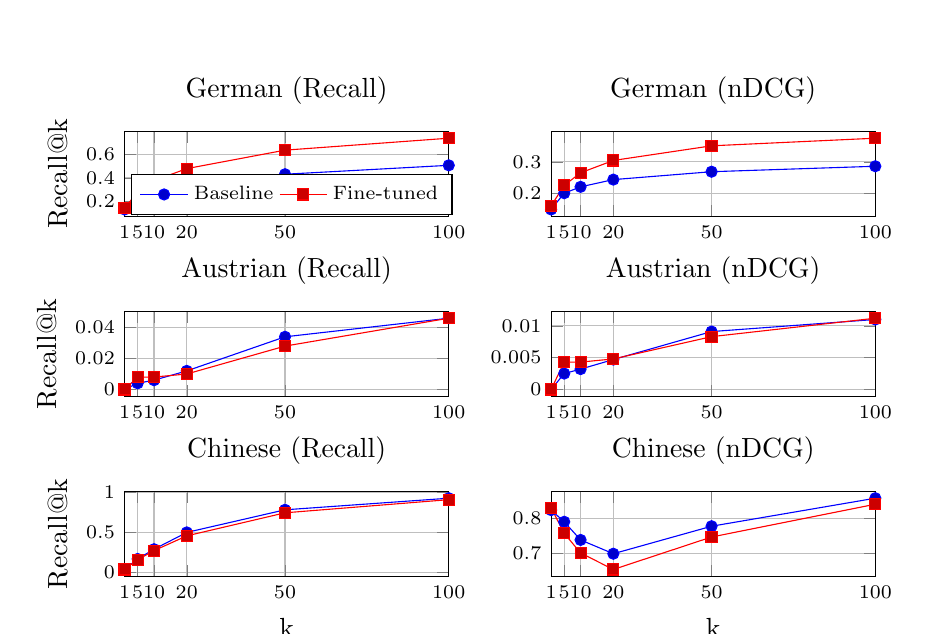
\begin{tikzpicture}
\begin{groupplot}[
  group style={group size=2 by 3, horizontal sep=1.3cm, vertical sep=1.2cm},
  width=0.47\textwidth,
  height=0.22\textwidth,
  xmin=1, xmax=100,
  xtick={1,5,10,20,50,100},
  xticklabels={1,5,10,20,50,100},
  xmode=normal,
  xlabel={},
  grid=both,
  scaled y ticks=false,
  tick label style={font=\scriptsize},
  yticklabel style={/pgf/number format/fixed, /pgf/number format/precision=3},
  title style={font=\normalsize},
  legend style={font=\scriptsize, draw=black, fill=white, at={(0.02,0.02)}, anchor=south west, legend columns=2},
  ylabel near ticks,
]

% Layout: rows = datasets (German/Austrian/Chinese), columns = metrics (Recall/nDCG)
\nextgroupplot[title={German (Recall)}, ylabel={Recall@k}]
\addplot+[mark=*] coordinates {(1,0.1330) (5,0.2343) (10,0.2826) (20,0.3436) (50,0.4313) (100,0.5066)};
\addplot+[mark=square*] coordinates {(1,0.1445) (5,0.2803) (10,0.3767) (20,0.4788) (50,0.6350) (100,0.7361)};
\legend{Baseline, Fine-tuned}

\nextgroupplot[title={German (nDCG)}, ylabel={}]
\addplot+[mark=*] coordinates {(1,0.1500) (5,0.2013) (10,0.2214) (20,0.2442) (50,0.2691) (100,0.2863)};
\addplot+[mark=square*] coordinates {(1,0.1615) (5,0.2260) (10,0.2657) (20,0.3046) (50,0.3508) (100,0.3748)};

\nextgroupplot[title={Austrian (Recall)}, ylabel={Recall@k}]
\addplot+[mark=*] coordinates {(1,0.0000) (5,0.0040) (10,0.0060) (20,0.0120) (50,0.0340) (100,0.0460)};
\addplot+[mark=square*] coordinates {(1,0.0000) (5,0.0080) (10,0.0080) (20,0.0100) (50,0.0280) (100,0.0460)};

\nextgroupplot[title={Austrian (nDCG)}, ylabel={}]
\addplot+[mark=*] coordinates {(1,0.0000) (5,0.0025) (10,0.0032) (20,0.0047) (50,0.0091) (100,0.0110)};
\addplot+[mark=square*] coordinates {(1,0.0000) (5,0.0043) (10,0.0043) (20,0.0048) (50,0.0083) (100,0.0112)};

\nextgroupplot[title={Chinese (Recall)}, xlabel={k}, ylabel={Recall@k}]
\addplot+[mark=*] coordinates {(1,0.0374) (5,0.1694) (10,0.2912) (20,0.5018) (50,0.7848) (100,0.9299)};
\addplot+[mark=square*] coordinates {(1,0.0380) (5,0.1597) (10,0.2737) (20,0.4585) (50,0.7472) (100,0.9118)};

\nextgroupplot[title={Chinese (nDCG)}, xlabel={k}, ylabel={}]
\addplot+[mark=*] coordinates {(1,0.8239) (5,0.7905) (10,0.7386) (20,0.6992) (50,0.7778) (100,0.8579)};
\addplot+[mark=square*] coordinates {(1,0.8302) (5,0.7575) (10,0.7013) (20,0.6542) (50,0.7470) (100,0.8407)};

\end{groupplot}
\end{tikzpicture}

\caption{Recall@k and nDCG@k trends for baseline vs fine-tuned across datasets.}
\label{fig:curves}
\end{figure}

\section{Detailed Results Tables}
Tables~\ref{tab:results-german}--\ref{tab:results-chinese} provide the full Recall@k, Precision@k, and nDCG@k results for all three datasets.

\begin{table}[h]
\centering
\setlength{\tabcolsep}{6pt}
\renewcommand{\arraystretch}{1.15}
\begin{tabular}{llrrrrrr}
\toprule
Setup & Metric & @1 & @5 & @10 & @20 & @50 & @100 \\
\midrule
\multirow{3}{*}{Baseline} & Recall & 0.1330 & 0.2343 & 0.2826 & 0.3436 & 0.4313 & 0.5066 \\
 & Precision & 0.1500 & 0.0544 & 0.0330 & 0.0204 & 0.0103 & 0.0060 \\
 & nDCG & 0.1500 & 0.2013 & 0.2214 & 0.2442 & 0.2691 & 0.2863 \\
\midrule
\multirow{3}{*}{Fine-tuned} & Recall & 0.1445 & 0.2803 & 0.3767 & 0.4788 & 0.6350 & 0.7361 \\
 & Precision & 0.1615 & 0.0643 & 0.0434 & 0.0280 & 0.0150 & 0.0087 \\
 & nDCG & 0.1615 & 0.2260 & 0.2657 & 0.3046 & 0.3508 & 0.3748 \\
\bottomrule
\end{tabular}
\caption{German retrieval results (GerDaLIRSmall test): baseline vs fine-tuned.}
\label{tab:results-german}
\end{table}

\begin{table}[h]
\centering
\setlength{\tabcolsep}{6pt}
\renewcommand{\arraystretch}{1.15}
\begin{tabular}{llrrrrrr}
\toprule
Setup & Metric & @1 & @5 & @10 & @20 & @50 & @100 \\
\midrule
\multirow{3}{*}{Baseline} & Recall & 0.0000 & 0.0040 & 0.0060 & 0.0120 & 0.0340 & 0.0460 \\
 & Precision & 0.0000 & 0.0008 & 0.0006 & 0.0006 & 0.0007 & 0.0005 \\
 & nDCG & 0.0000 & 0.0025 & 0.0032 & 0.0047 & 0.0091 & 0.0110 \\
\midrule
\multirow{3}{*}{Fine-tuned} & Recall & 0.0000 & 0.0080 & 0.0080 & 0.0100 & 0.0280 & 0.0460 \\
 & Precision & 0.0000 & 0.0016 & 0.0008 & 0.0005 & 0.0006 & 0.0005 \\
 & nDCG & 0.0000 & 0.0043 & 0.0043 & 0.0048 & 0.0083 & 0.0112 \\
\bottomrule
\end{tabular}
\caption{Austrian retrieval results (synthetic): baseline vs fine-tuned.}
\label{tab:results-austrian}
\end{table}

\begin{table}[h]
\centering
\setlength{\tabcolsep}{6pt}
\renewcommand{\arraystretch}{1.15}
\begin{tabular}{llrrrrrr}
\toprule
Setup & Metric & @1 & @5 & @10 & @20 & @50 & @100 \\
\midrule
\multirow{3}{*}{Baseline} & Recall & 0.0374 & 0.1694 & 0.2912 & 0.5018 & 0.7848 & 0.9299 \\
 & Precision & 0.8239 & 0.7585 & 0.6780 & 0.5972 & 0.3824 & 0.2275 \\
 & nDCG & 0.8239 & 0.7905 & 0.7386 & 0.6992 & 0.7778 & 0.8579 \\
\midrule
\multirow{3}{*}{Fine-tuned} & Recall & 0.0380 & 0.1597 & 0.2737 & 0.4585 & 0.7472 & 0.9118 \\
 & Precision & 0.8302 & 0.7182 & 0.6296 & 0.5472 & 0.3638 & 0.2233 \\
 & nDCG & 0.8302 & 0.7575 & 0.7013 & 0.6542 & 0.7470 & 0.8407 \\
\bottomrule
\end{tabular}
\caption{Chinese retrieval results (LeCaRDv2 test): baseline vs fine-tuned.}
\label{tab:results-chinese}
\end{table}

\newpage
\section{Workflow Diagram}
Figure~\ref{fig:flowchart} shows the workflow from data collection to evaluation.

\begin{figure}[h]
\centering
\includegraphics[width=\textwidth]{../design-document/flowchart.pdf}
\caption{Project workflow and methodology.}
\label{fig:flowchart}
\end{figure}

\newpage
\printbibliography
\end{document}

